\emph{Inteligencia artificial} es definida como ``el esfuerzo por automatizar tareas intelectuales normalmente realizadas por humanos''\cite{cho18}, de este campo general se desprenden el \emph{aprendizaje maquinal} y el \emph{aprendizaje profundo}.

\begin{figure}[H]\centering
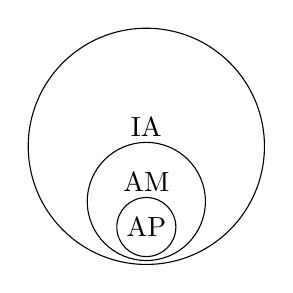
\begin{tikzpicture}
\def\IA{(0,0) circle (1.5cm)}
\def\AM{(270:.7cm) circle (.75cm)}
\def\AP{(270:1.025cm) circle (.375cm)}
\draw \IA node[above]{IA};
\draw \AM node[above]{AM};
\draw \AP node{AP};
\end{tikzpicture}
\caption{Aprendizaje profundo (AP), es un subcampo del aprendizaje maquinal (AM), que a su vez es un subcampo de la inteligencia artificial (IA)\cite{cho18}.}\label{fig:AI}
\end{figure}